\documentclass{standalone}
\usepackage{graphicx}	
\usepackage{amssymb, amsmath, amsthm}
\usepackage{color}

\usepackage{tikz}
\usetikzlibrary{intersections, backgrounds}

\definecolor{light}{RGB}{220, 188, 188}
\definecolor{mid}{RGB}{185, 124, 124}
\definecolor{dark}{RGB}{143, 39, 39}
\definecolor{gray80}{gray}{0.8}
\definecolor{gray90}{gray}{0.90}
\definecolor{gray95}{gray}{0.95}

\begin{document}

\begin{tikzpicture}[scale=0.25, thick]
  \draw[-,color=white] (-12, 0) to (12, 0);
  
  \begin{scope}
  \clip (-12, -8) rectangle (12, 11);
  
  \foreach \i in {1, 0.99, ..., 0} {
    \pgfmathsetmacro{\prop}{100 * exp(-10.0 * \i * \i)};
    \colorlet{custom}{dark!\prop!white};
    \draw[line width={30 * \i}, color=custom] 
      (-10, 0) .. controls (-10, 15) and (-5, 5) .. (0, 5)
      .. controls (5, 5) and (10, 8) .. (10, 0)
      .. controls (10, -8) and (5, -3) .. (0, -3)
      .. controls (-5, -3) and (-10, -5) .. (-10, 0);
  }

  \fill[color=dark] (-11, -7.75) circle (7pt);  
  \fill[color=light] (-11, -7.75) circle (5pt);
  
  \fill[color=dark] (-10, -6.5) circle (7pt);  
  \fill[color=light] (-10, -6.5) circle (5pt);
  
  \fill[color=dark] (-9, -6.75) circle (7pt);  
  \fill[color=light] (-9, -6.75) circle (5pt);
  
  \fill[color=dark] (-8.25, -5) circle (7pt);  
  \fill[color=light] (-8.25, -5) circle (5pt);
  
  \fill[color=dark] (-7.5, -4) circle (7pt);  
  \fill[color=light] (-7.5, -4) circle (5pt);
  
  \fill[color=dark] (-7, -3.5) circle (7pt);  
  \fill[color=light] (-7, -3.5) circle (5pt);
  
  \fill[color=dark] (-6.5, -3.6) circle (7pt);  
  \fill[color=light] (-6.5, -3.6) circle (5pt);  
  
  \end{scope}
  
  \draw[-,color=white] (14, 0) to (38, 0);  
  \node[] at (28, 0.5) {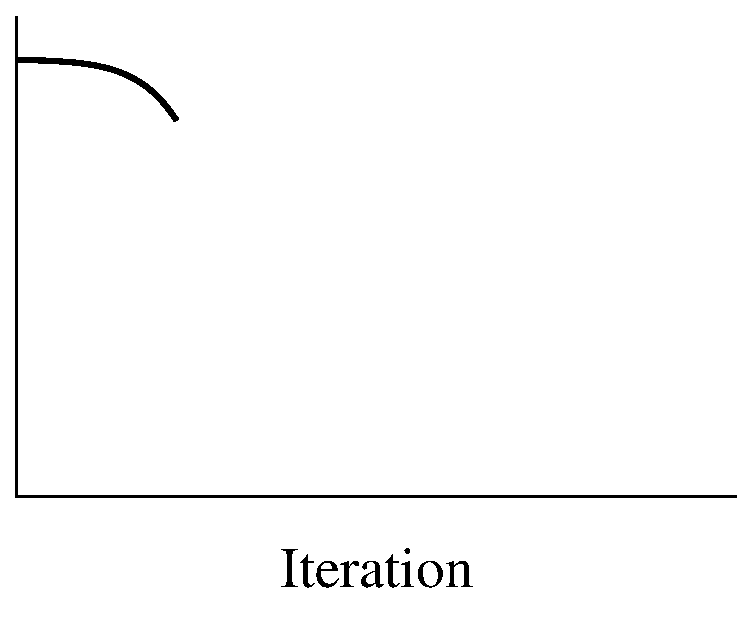
\includegraphics[width=5cm]{gnuplot/convergence1.eps}};
  \node[rotate=90] at (16.25, 1.75) { $\left| \mathbb{E} \! \left[ f \right] - \hat{f} \right|$ };
\end{tikzpicture}

\end{document}  